\documentclass{article}
\usepackage[utf8]{inputenc}
\usepackage{amsmath}
\usepackage{amssymb}
\usepackage{graphicx}
\usepackage{tabularx}
\usepackage{booktabs}
\usepackage[english]{babel}
\usepackage{setspace}
\usepackage{geometry}
\usepackage{float}
\usepackage{url}
\usepackage{listings}
\usepackage{xcolor}
\usepackage{longtable}
\usepackage{tikz}
\usetikzlibrary{positioning, calc}
\usepackage[justification=centering]{caption}

\lstset{
    basicstyle=\ttfamily\small,
    backgroundcolor=\color{gray!10},
    frame=single,
    breaklines=true,
    columns=fullflexible
}

% APA style formatting
\geometry{a4paper, margin=1in}
\setstretch{1.5}
\setlength{\emergencystretch}{3em} % lets long \texttt names wrap without overflowing the margin
\captionsetup[table]{labelfont=bf, justification=centering, singlelinecheck=false}
\captionsetup[longtable]{labelfont=bf, justification=centering, singlelinecheck=false}
\captionsetup[figure]{font=small, labelfont=bf, justification=centering, singlelinecheck=false}

% Notation helpers
\newcommand{\R}{\mathbb{R}}
\newcommand{\slog}{\operatorname{slog}}
\newcommand{\clip}{\operatorname{clip}}
\newcommand{\ind}{\mathbf{1}}

\title{Machine Learning for Customer Churn Prediction}
\author{Nelson David Posso Suarez \\ Javier Alejandro Penagos Hernandez \\ Nicolas Castro Rivera }
\date{}

\begin{document}

\maketitle

% ─────────────────────────────────────────────
\section{Data Preparation}
% ─────────────────────────────────────────────

In this workshop the churn problem is approached from a different angle. Instead of summarising each subscriber into a single tabular row, as in Workshop~1, we use the dates in the dataset to treat churn prediction as a \textbf{sequence problem}: each subscriber is represented by the day-by-day evolution of their listening activity and subscription status. This requires transforming the raw data in a different way from the previous workshop. The pipeline is implemented in \path{workshops/w2/w2_sequence_preprocessing.ipynb} and the modules under \path{workshops/w2/src/data_processing/}.

% ─────────────────────────────────────────────
\subsection{Structure of the Raw Data}
% ─────────────────────────────────────────────

The dataset was obtained from the \emph{WSDM--KKBox's Churn Prediction Challenge}, hosted on Kaggle in 2017 with data donated by KKBOX \cite{kkbox2017}. It covers approximately 2015 to 2017 and contains the history of each subscriber's transactions and music listening logs. Three of the raw tables are used to build the sequences: the labelled cohorts (Table~\ref{tab:w2_schema_train}), the daily listening logs (Table~\ref{tab:w2_schema_logs}) and the payment transactions (Table~\ref{tab:w2_schema_transactions}). The member demographics table is not used in this workshop.

\begin{table}[H]
\centering
\renewcommand{\arraystretch}{1.3}
\begin{tabularx}{\textwidth}{|l|X|l|}
\hline
\textbf{Feature} & \textbf{Description} & \textbf{Data type} \\ \hline
msno      & Hashed subscriber identifier (primary key) & \texttt{str} \\ \hline
is\_churn & Churn label: 1 if the user did not renew within 30 days of expiry, 0 otherwise & \texttt{int8} \\ \hline
\end{tabularx}
\caption{Schema of \texttt{train.csv} (February cohort) and \texttt{train\_v2.csv} (March cohort).}
\label{tab:w2_schema_train}
\end{table}

\begin{table}[H]
\centering
\renewcommand{\arraystretch}{1.3}
\begin{tabularx}{\textwidth}{|l|X|l|}
\hline
\textbf{Feature} & \textbf{Description} & \textbf{Data type} \\ \hline
msno        & Hashed subscriber identifier (foreign key) & \texttt{str} \\ \hline
date        & Listening date in YYYYMMDD format & \texttt{int32} \\ \hline
num\_25     & Number of songs played less than 25\% of their duration & \texttt{int32} \\ \hline
num\_50     & Number of songs played between 25\% and 50\% of their duration & \texttt{int32} \\ \hline
num\_75     & Number of songs played between 50\% and 75\% of their duration & \texttt{int32} \\ \hline
num\_985    & Number of songs played between 75\% and 98.5\% of their duration & \texttt{int32} \\ \hline
num\_100    & Number of songs played at least 98.5\% of their duration & \texttt{int32} \\ \hline
num\_unq    & Number of unique songs played on that day & \texttt{int32} \\ \hline
total\_secs & Total seconds of music listened to on that day & \texttt{float64} \\ \hline
\end{tabularx}
\caption{Schema of \texttt{user\_logs.csv} and \texttt{user\_logs\_v2.csv}.}
\label{tab:w2_schema_logs}
\end{table}

\begin{table}[H]
\centering
\renewcommand{\arraystretch}{1.3}
\begin{tabularx}{\textwidth}{|l|X|l|}
\hline
\textbf{Feature} & \textbf{Description} & \textbf{Data type} \\ \hline
msno                     & Hashed subscriber identifier (foreign key) & \texttt{str} \\ \hline
payment\_method\_id      & Payment method encoded as an integer code & \texttt{int8} \\ \hline
payment\_plan\_days      & Number of days in the purchased subscription plan & \texttt{int16} \\ \hline
plan\_list\_price        & Listed price of the plan in New Taiwan Dollars (NTD) & \texttt{int16} \\ \hline
actual\_amount\_paid     & Amount actually paid by the subscriber in NTD & \texttt{int16} \\ \hline
is\_auto\_renew          & Automatic renewal flag (1 = yes, 0 = no) & \texttt{int8} \\ \hline
transaction\_date        & Date of the transaction in YYYYMMDD format & \texttt{int32} \\ \hline
membership\_expire\_date & Membership expiration date after the transaction in YYYYMMDD format & \texttt{int32} \\ \hline
is\_cancel               & Cancellation flag (1 = yes, 0 = no) & \texttt{int8} \\ \hline
\end{tabularx}
\caption{Schema of \texttt{transactions.csv} and \texttt{transactions\_v2.csv}.}
\label{tab:w2_schema_transactions}
\end{table}

% ─────────────────────────────────────────────
\subsection{Tensor Construction}
% ─────────────────────────────────────────────

\subsubsection{Temporal Split and Window Overlap}

Each cohort $c$ is defined by a cutoff date $\tau_c$, the last day whose information may be used. Its sequence window contains the $L = 90$ consecutive calendar days that end on the cutoff:
\begin{equation}
W_c = \{\, \tau_c - 89,\; \tau_c - 88,\; \dots,\; \tau_c \,\}, \qquad |W_c| = L = 90 .
\end{equation}
A calendar date $d \in W_c$ is mapped to the day index
\begin{equation}
t(d) = d - (\tau_c - 89) \in \{0, 1, \dots, 89\},
\end{equation}
so $t = 0$ is the oldest day of the window and $t = 89$ is the cutoff. Table~\ref{tab:w2_cohorts} lists the two cohorts.

\begin{table}[H]
\centering
\renewcommand{\arraystretch}{1.3}
\begin{tabular}{|l|l|l|l|r|r|}
\hline
\textbf{Cohort} & \textbf{Role} & \textbf{Window $W_c$} & \textbf{Target} & \textbf{Users $N_c$} & \textbf{Churn rate} \\ \hline
\texttt{train\_feb} & Training & 2016-11-03 to 2017-01-31 & February 2017 & 992{,}931 & 6.4\% \\ \hline
\texttt{test}       & Test     & 2016-12-01 to 2017-02-28 & March 2017    & 970{,}960 & 9.0\% \\ \hline
\end{tabular}
\caption{Labelled cohorts, their 90-day windows and churn targets.}
\label{tab:w2_cohorts}
\end{table}

We build the training tensor from each user's activity between 2016-11-03 and 2017-01-31, with February 2017 churn as the target. The test tensor uses the window from 2016-12-01 to 2017-02-28, with March 2017 churn as the target. The two windows overlap by 62 days (2016-12-01 to 2017-01-31), as shown in Figure~\ref{fig:w2_overlap}.

\begin{figure}[H]
\centering
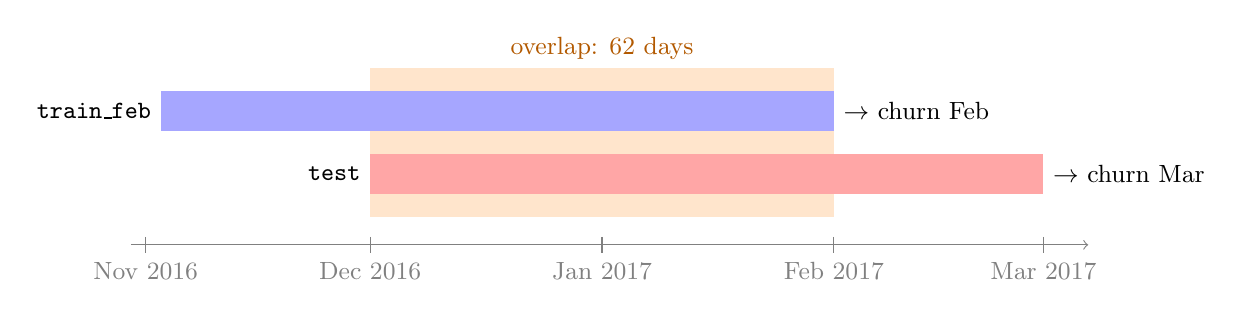
\begin{tikzpicture}[x=0.095cm, y=1cm, font=\small]
    % Day 0 = 2016-11-03. Month starts: Nov 1 = -2, Dec 1 = 28, Jan 1 = 59, Feb 1 = 90, Mar 1 = 118
    \draw[->, gray] (-4,0) -- (124,0);
    \foreach \x/\lbl in {-2/Nov 2016, 28/Dec 2016, 59/Jan 2017, 90/Feb 2017, 118/Mar 2017} {
        \draw[gray] (\x,0.1) -- (\x,-0.1);
        \node[below, gray] at (\x,-0.1) {\lbl};
    }
    % Overlap band
    \fill[orange!20] (28,0.35) rectangle (90,2.25);
    \node[orange!70!black] at (59,2.5) {overlap: 62 days};
    % Train window
    \fill[blue!35] (0,1.45) rectangle (90,1.95);
    \node[left] at (0,1.7) {\texttt{train\_feb}};
    \node[right] at (90,1.7) {$\rightarrow$ churn Feb};
    % Test window
    \fill[red!35] (28,0.65) rectangle (118,1.15);
    \node[left] at (28,0.9) {\texttt{test}};
    \node[right] at (118,0.9) {$\rightarrow$ churn Mar};
\end{tikzpicture}
\caption{90-day windows of the two cohorts. Each window ends at its cutoff (2017-01-31 and 2017-02-28) and is followed by its target month.}
\label{fig:w2_overlap}
\end{figure}

This overlap is intentional. It follows from using a fixed-length lookback window that advances one month at a time, which is how a subscription service would score its customers in production. Each month, the model receives the most recent 90 days of behaviour and predicts whether the customer will renew in the following month, so consecutive scoring windows necessarily share most of their history.

The overlap does not leak target information. Every feature is computed using only data up to its window's cutoff, and the labels belong to different, non-overlapping periods (February for training, March for testing). During training the model never observes the March outcome, nor any activity after 2017-01-31. The test set therefore measures forward-looking temporal generalisation: how well a model trained on one month's snapshot predicts the next month's churn, including any behavioural drift between the two months.

Many users appear in both cohorts (881{,}701 of the February users are also in the March cohort), as they would in real monthly scoring. A shared integer identifier \texttt{uid} is assigned over the union of both cohorts (1{,}082{,}190 unique users) and is used only to join each user with their logs and transactions. Each cohort keeps its own complete list of users, its own row order and its own labels: a user present in only one cohort appears only in that cohort's tensor, and a user present in both appears twice, with a different cutoff, sequence and label each time. Our results should therefore be read as performance on an existing customer base rather than on entirely unseen users.

\subsubsection{Cleaning}

\paragraph{Transactions.} Both transaction files are concatenated, restricted to the target users and to transactions on or before the cutoff. Exact duplicates are then removed: two rows are considered duplicates when the user (\texttt{msno}) and all eight transaction fields (\texttt{payment\_method\_id}, \texttt{payment\_plan\_days}, \texttt{plan\_list\_price}, \texttt{actual\_amount\_paid}, \texttt{is\_auto\_renew}, \texttt{transaction\_date}, \texttt{membership\_expire\_date}, \texttt{is\_cancel}) are equal. Only the first copy is kept. Two rows on the same day with different values are treated as different payments and both are kept.

\paragraph{Listening logs.} The raw logs may contain several rows for the same user and day. Before aggregation, negative counters are clipped to zero and non-finite values of \texttt{total\_secs} are replaced by zero. The rows of the same user and day are then summed into a single row. For example, if user $A$ has three rows on 2017-02-01, with \texttt{num\_25} equal to 3, 2 and 1, the aggregated row has \texttt{num\_25} $= 6$; the other counters are summed in the same way. Formally, for user $i$, day $d$ and counter $k$:
\begin{equation}
v_{i,d,k} = \sum_{r \in R_{i,d}} \max(0,\, v_{r,k}),
\end{equation}
where $R_{i,d}$ is the set of raw log rows of user $i$ on day $d$. The number of raw rows $|R_{i,d}|$ is kept to define the activity flag.

\subsubsection{Listening Channels}

The aggregated logs are placed into the window. Days without any log row are filled with zeros. The seven counters are transformed with $\log(1+x)$ to compress their heavy-tailed distribution; standard scaling is fitted later, on the training split only, inside the model notebook. An eighth channel, \texttt{active}, indicates whether a log row exists for that day, independently of the counter values:
\begin{equation}
x_{i,t,k} = \log\!\left(1 + v_{i,d,k}\right), \quad k = 1,\dots,7, \qquad
a_{i,t} = \ind\!\left[\,|R_{i,d}| > 0\,\right],
\end{equation}
with $t = t(d)$. A day with a log row where every counter is zero is still active, which distinguishes ``logged in but did not listen'' from ``no record''. Table~\ref{tab:w2_listening} lists the listening channels.

\begin{table}[H]
\centering
\renewcommand{\arraystretch}{1.3}
\begin{tabularx}{\textwidth}{|c|l|X|l|}
\hline
\textbf{Index} & \textbf{Channel} & \textbf{Description} & \textbf{Encoding} \\ \hline
0 & num\_25     & Songs played less than 25\% & $\log(1+x)$ \\ \hline
1 & num\_50     & Songs played 25--50\%       & $\log(1+x)$ \\ \hline
2 & num\_75     & Songs played 50--75\%       & $\log(1+x)$ \\ \hline
3 & num\_985    & Songs played 75--98.5\%     & $\log(1+x)$ \\ \hline
4 & num\_100    & Songs played at least 98.5\% & $\log(1+x)$ \\ \hline
5 & num\_unq    & Unique songs played         & $\log(1+x)$ \\ \hline
6 & total\_secs & Seconds listened            & $\log(1+x)$ \\ \hline
7 & active      & 1 if a log row exists for the day, 0 otherwise & flag \\ \hline
\end{tabularx}
\caption{Listening channels (8) of the sequence tensor.}
\label{tab:w2_listening}
\end{table}

\subsubsection{Transaction Channels: Events and States}

The tensor is completed with twelve transaction channels, divided into two groups:

\begin{itemize}
    \item \textbf{Events} encode what happened on a specific day. They are written only on the days with at least one payment and are zero on every other day.
    \item \textbf{States} encode the subscription status known at the end of a specific day. They are carried forward to the following days until the next payment updates them.
\end{itemize}

First, the transactions of each user are aggregated per day. Event values are summed over all payments of the day. State values (cancellation, auto-renewal and expiry date) are taken from the last record of that day in source order, and a flag marks the day as ambiguous when the records of the same day disagree on any of these three values.

\paragraph{Payments before the window.} Only the \textbf{latest payment day before the window} is kept from the earlier history; all earlier payments are summarised by that single record. This record initialises the state at $t = 0$ but does not create an event inside the window. A payment on day $t$ writes the event channels on day $t$ and updates the state from day $t$ onward. Future payments never modify earlier days, which guarantees that the tensor is causal. This property is verified in the notebook by comparing the vectorised builder against a day-by-day reference implementation and checking that adding a later payment leaves every earlier day unchanged.

Formally, let $P_i$ be the set of payment days of user $i$ up to the cutoff, and let
\begin{equation}
s_i(t) = \max \{\, p \in P_i : p \le d_t \,\}
\end{equation}
be the most recent payment day known on day $d_t$ (possibly before the window). The state is known when $s_i(t)$ exists, and the recency and expiry channels are
\begin{align}
\text{tx\_days\_since\_last}_{i,t} &= \log\!\Big(1 + \clip\big(d_t - s_i(t),\, 0,\, 3650\big)\Big), \\
\text{tx\_days\_to\_expire}_{i,t}  &= \slog\!\Big(\clip\big(e_i(t) - d_t,\, -3650,\, 3650\big)\Big),
\end{align}
where $e_i(t)$ is the membership expiry date recorded on day $s_i(t)$, and $\slog(x) = \operatorname{sign}(x)\log(1 + |x|)$ is the signed logarithm, used for quantities that can be negative (an already expired membership, or a negative amount paid). When the state is not yet known, all state channels are zero.

\paragraph{Worked example.} Consider a user of the \texttt{test} cohort, whose window starts on 2016-12-01 ($t = 0$). The user paid on 2016-11-20, before the window, with auto-renewal disabled and a membership that expires on 2016-12-20, and made no further payments. The pre-window payment initialises the state, so $s_i(t) = \text{2016-11-20}$ and $e_i(t) = \text{2016-12-20}$ for every day of the window, and no event is written on any day. Table~\ref{tab:w2_example} shows the two channels on three days. On day 19 the membership expires and \texttt{tx\_days\_to\_expire} is zero; from day 20 on it is negative, a strong signal that the user has not renewed. These values were obtained by running this user through the same builder used for the export.

\begin{table}[H]
\centering
\renewcommand{\arraystretch}{1.3}
\begin{tabular}{|c|c|c|c|c|c|}
\hline
\textbf{Day $t$} & \textbf{Date $d_t$} & $d_t - s_i(t)$ & \textbf{tx\_days\_since\_last} & $e_i(t) - d_t$ & \textbf{tx\_days\_to\_expire} \\ \hline
0  & 2016-12-01 & 11 & $\log(1 + 11) = 2.48$ & 19  & $\slog(19) = 3.00$ \\ \hline
19 & 2016-12-20 & 30 & $\log(1 + 30) = 3.43$ & 0   & $\slog(0) = 0.00$ \\ \hline
24 & 2016-12-25 & 35 & $\log(1 + 35) = 3.58$ & $-5$ & $\slog(-5) = -1.79$ \\ \hline
\end{tabular}
\caption{Recency and expiry channels for a user whose only payment (2016-11-20, expiring 2016-12-20) falls before the \texttt{test} window.}
\label{tab:w2_example}
\end{table}

Table~\ref{tab:w2_transactions} describes each transaction channel.

\renewcommand{\arraystretch}{1.3}
\begin{longtable}{|c|l|c|p{6.2cm}|l|}
\hline
\textbf{Index} & \textbf{Channel} & \textbf{Group} & \textbf{Description} & \textbf{Encoding} \\ \hline
\endfirsthead
\hline
\textbf{Index} & \textbf{Channel} & \textbf{Group} & \textbf{Description} & \textbf{Encoding} \\ \hline
\endhead
\hline
\multicolumn{5}{r}{\small\textit{Continued on next page}} \\
\endfoot
\hline
\caption{Transaction channels (12) of the sequence tensor.}
\label{tab:w2_transactions}
\endlastfoot
8  & tx\_count               & Event & Number of payments on the day & $\log(1+x)$ \\ \hline
9  & tx\_paid\_sum           & Event & Total amount paid on the day (NTD) & $\slog(x)$ \\ \hline
10 & tx\_plan\_days\_sum     & Event & Total plan days purchased on the day & $\log(1+x)$ \\ \hline
11 & tx\_cancel\_count       & Event & Number of cancellation records on the day & $\log(1+x)$ \\ \hline
12 & tx\_auto\_renew\_count  & Event & Number of auto-renew records on the day & $\log(1+x)$ \\ \hline
13 & tx\_state\_known        & State & 1 once at least one payment has been observed up to the day, including the pre-window payment & flag \\ \hline
14 & tx\_last\_is\_cancel    & State & Cancellation flag of the most recent payment day & flag \\ \hline
15 & tx\_last\_is\_auto\_renew & State & Auto-renew flag of the most recent payment day & flag \\ \hline
16 & tx\_days\_since\_last   & State & Days since the most recent payment, clipped to $[0, 3650]$ & $\log(1+x)$ \\ \hline
17 & tx\_days\_to\_expire    & State & Membership expiry minus the current day, clipped to $[-3650, 3650]$ & $\slog(x)$ \\ \hline
18 & tx\_expiry\_known       & State & 1 if the expiry date of the most recent payment is valid & flag \\ \hline
19 & tx\_state\_ambiguous    & State & 1 if the records of the most recent payment day disagree on cancellation, auto-renewal or expiry & flag \\ \hline
\end{longtable}

\subsubsection{Resulting Tensor}

For each user $i$ of cohort $c$, the 20 channels are stacked into a matrix whose rows are the 90 days, ordered from oldest to newest, and whose columns are the channels in the order of Tables~\ref{tab:w2_listening} and~\ref{tab:w2_transactions}:
\begin{equation}
X_i^{(c)} =
\begin{bmatrix}
x_{i,0,0}  & x_{i,0,1}  & \cdots & x_{i,0,19} \\
x_{i,1,0}  & x_{i,1,1}  & \cdots & x_{i,1,19} \\
\vdots     & \vdots     & \ddots & \vdots \\
x_{i,89,0} & x_{i,89,1} & \cdots & x_{i,89,19}
\end{bmatrix}
\in \R^{L \times F}, \qquad L = 90,\; F = 20 .
\end{equation}
Stacking the $N_c$ users of the cohort gives the cohort tensor
\begin{equation}
\mathcal{X}^{(c)} = \big[\, X_1^{(c)}, X_2^{(c)}, \dots, X_{N_c}^{(c)} \,\big] \in \R^{N_c \times L \times F},
\end{equation}
together with the label vector $y^{(c)} \in \{0,1\}^{N_c}$, aligned so that position $i$ of $y^{(c)}$ is the label of $X_i^{(c)}$. The channel dimension splits into three blocks:
\begin{equation}
X_i^{(c)} = \big[\; \underbrace{X_i^{\text{listen}}}_{\R^{90 \times 8}} \;\big|\; \underbrace{X_i^{\text{event}}}_{\R^{90 \times 5}} \;\big|\; \underbrace{X_i^{\text{state}}}_{\R^{90 \times 7}} \;\big].
\end{equation}

In this way we obtain $\mathcal{X}^{(\text{train\_feb})} \in \R^{992{,}931 \times 90 \times 20}$ and $\mathcal{X}^{(\text{test})} \in \R^{970{,}960 \times 90 \times 20}$. The tensors are stored as \texttt{float16} arrays (\texttt{seq\_lstm\_train\_feb.npy} and \texttt{seq\_lstm\_test.npy}, about 3.5~GB each) with their labels in \texttt{labels\_<cohort>.parquet}, in the directory \texttt{workshops/w2/export-sequential-v5/}. Before export, an audit rejects the tensor if any of the following fails: the expected shape, finite values, binary flags, non-negative counts and recency, zero event channels on days without a payment, and zero state channels before the state is known.

% ─────────────────────────────────────────────
\section{Recurrent Models}
% ─────────────────────────────────────────────

We compare two gated recurrent neural networks: a Long Short-Term Memory network (LSTM) and a Gated Recurrent Unit network (GRU). Both read the 90 days in chronological order and maintain a hidden representation of the customer's behaviour. Prior empirical work found GRU performance comparable to LSTM on sequence-modelling tasks, while noting that the relative result depends on the dataset and task \cite{chung2014}. Our comparison isolates the recurrent cell: the input tensor, preprocessing, data partitions, classifier head, loss, optimiser, search space and evaluation protocol are identical. The models are implemented in PyTorch by the shared \texttt{RecurrentClassifier} and its subclasses \texttt{LSTMModel} and \texttt{GRUModel} (\path{workshops/w2/src/models/recurrent_models/recurrent_classifier.py}); training and evaluation are orchestrated in \path{workshops/w2/w2_neural_models.ipynb}.

\subsection{Architecture}

The common architecture has the following layers (Figure~\ref{fig:w2_arch}):

\begin{itemize}
    \item \textbf{Input layer.} A batch of users taken from the tensor built before, with shape $(B, 90, 20)$: $B$ users, 90 days and 20 channels. Each day $t$ of user $i$ is the vector $x_{i,t} \in \R^{20}$.
    \item \textbf{Recurrent encoder.} Either stacked LSTM or stacked GRU layers. The first layer reads the 20 channels and each subsequent layer reads the hidden states of the layer below.
    \item \textbf{Hidden dimension} (\texttt{hidden\_dim}). The number of units in each hidden state $h_t \in \R^{H}$; it controls the capacity of the temporal representation.
    \item \textbf{Layer dimension} (\texttt{layer\_dim}). The number of stacked recurrent layers, between 2 and 4.
    \item \textbf{Batch normalisation layer.} After the 90 days, the output of the last layer on the last day, $h_{90} \in \R^{H}$, has shape $(B, H)$. This vector summarises the customer's behaviour over the 90 days. \texttt{BatchNorm1d} normalises it across the batch, which stabilises the training.
    \item \textbf{Output layer.} A linear layer applies the transformation $z = w^\top \tilde{h}_{90} + b$ and produces one value per user, the \emph{logit} $z \in \R$.
\end{itemize}

\subsubsection{LSTM Cell}

For each day, an LSTM cell updates a separate memory cell $c_t$ and hidden state $h_t$ with
\begin{align}
f_t &= \sigma(W_f x_t + U_f h_{t-1} + b_f), &
i_t &= \sigma(W_i x_t + U_i h_{t-1} + b_i), &
o_t &= \sigma(W_o x_t + U_o h_{t-1} + b_o), \\
\tilde{c}_t &= \tanh(W_c x_t + U_c h_{t-1} + b_c), &
c_t &= f_t \odot c_{t-1} + i_t \odot \tilde{c}_t, &
h_t &= o_t \odot \tanh(c_t),
\end{align}
where $f_t$, $i_t$ and $o_t$ are the forget, input and output gates, $\sigma$ is the sigmoid function and $\odot$ is the element-wise product. The states start at $h_0 = c_0 = 0$.

The explicit memory path allows the forget gate to retain information over many time steps, while the input and output gates control what is written and exposed. This flexibility comes at a computational cost: each layer computes four affine transformations (three gates and one candidate state).

\subsubsection{GRU Cell}

The GRU merges the memory and hidden states into a single vector. For each day it computes a reset gate $r_t$, an update gate $u_t$ and a candidate state $n_t$:
\begin{align}
r_t &= \sigma(W_r x_t + U_r h_{t-1} + b_r), \\
u_t &= \sigma(W_u x_t + U_u h_{t-1} + b_u), \\
n_t &= \tanh\!\left(W_n x_t + b_n + r_t \odot (U_n h_{t-1} + d_n)\right), \\
h_t &= (1-u_t) \odot n_t + u_t \odot h_{t-1}.
\end{align}
The reset gate controls how much previous information enters the candidate, and the update gate interpolates between the new candidate and the previous state. Thus, when $u_t$ is close to one, the GRU preserves its previous memory; when it is close to zero, it replaces it with the candidate. A GRU uses three affine transformations instead of the LSTM's four and has no separate cell state, so it is generally smaller and faster for the same $H$ and number of layers.

For either encoder, the states start at zero and the classifier uses only the final hidden state. The model output and churn probability are
\begin{equation}
z_i = w^\top \operatorname{BN}\big(h_{i,90}\big) + b, \qquad \hat{p}_i = \sigma(z_i) = \frac{1}{1 + e^{-z_i}} .
\end{equation}

\begin{figure}[H]
\centering
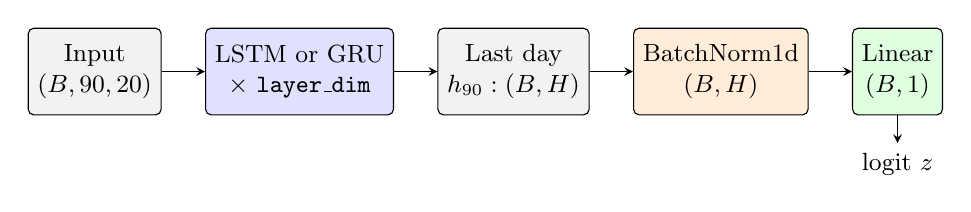
\begin{tikzpicture}[
    box/.style={draw, rounded corners=2pt, minimum height=1.1cm, align=center, font=\small, fill=#1},
    box/.default={gray!10},
    >=stealth, node distance=0.55cm
]
    \node[box] (in) {Input\\$(B, 90, 20)$};
    \node[box=blue!12, right=of in] (rnn) {LSTM or GRU\\$\times$ \texttt{layer\_dim}};
    \node[box, right=of rnn] (last) {Last day\\$h_{90}: (B, H)$};
    \node[box=orange!15, right=of last] (bn) {BatchNorm1d\\$(B, H)$};
    \node[box=green!12, right=of bn] (fc) {Linear\\$(B, 1)$};
    \draw[->] (in) -- (rnn);
    \draw[->] (rnn) -- (last);
    \draw[->] (last) -- (bn);
    \draw[->] (bn) -- (fc);
    \node[below=0.35cm of fc, font=\small] (out) {logit $z$};
    \draw[->] (fc) -- (out);
\end{tikzpicture}
\caption{Common LSTM/GRU classifier architecture. Only the recurrent cell changes between models; $B$ is the batch size and $H$ the hidden dimension.}
\label{fig:w2_arch}
\end{figure}

\subsection{Loss Function and Optimiser}

Since churn is a binary classification problem, we use the binary cross-entropy loss. In PyTorch it is defined as \texttt{criterion = nn.BCEWithLogitsLoss()}. This function receives the logit $z_i$ and applies the sigmoid internally, so the model does not include a sigmoid layer. Combining both operations in one function is numerically stable: it never evaluates $\log(0)$ when the sigmoid saturates. For a batch of $B$ users the loss is
\begin{equation}
\mathcal{L} = -\frac{1}{B} \sum_{i=1}^{B} \Big[ y_i \log \sigma(z_i) + (1 - y_i) \log\big(1 - \sigma(z_i)\big) \Big].
\end{equation}
At prediction time, where there is no loss, the probability is obtained explicitly with \path{torch.sigmoid(logits)}.

\paragraph{Backpropagation.} Training needs the gradient of the loss with respect to every weight $\theta$ of the network. Backpropagation computes it by applying the chain rule backwards, from the loss to the input, through the same operations used in the forward pass (Figure~\ref{fig:w2_backprop}). Using the derivative of the sigmoid, $\sigma'(z) = \sigma(z)\big(1 - \sigma(z)\big)$, the first two steps for one user are
\begin{equation}
\frac{\partial \mathcal{L}}{\partial \hat p} = -\frac{y}{\hat p} + \frac{1 - y}{1 - \hat p},
\qquad
\frac{\partial \mathcal{L}}{\partial z} = \frac{\partial \mathcal{L}}{\partial \hat p} \cdot \sigma'(z) = \frac{\hat p - y}{\hat p (1 - \hat p)} \cdot \hat p (1 - \hat p) = \hat p - y .
\end{equation}
The derivative of the sigmoid cancels the denominator of the cross-entropy, so the error signal that enters the network is simply the difference between the predicted probability and the true label. It is large when the prediction is confidently wrong and close to zero when it is correct, and the saturation of the sigmoid cannot make it vanish while the prediction is wrong. This simplification is also what \texttt{BCEWithLogitsLoss} exploits to compute the loss and its gradient in a stable way. From $z$, the gradient continues to the output layer and to the hidden state:
\begin{equation}
\frac{\partial \mathcal{L}}{\partial w} = (\hat p - y)\, \tilde h_{90}, \qquad
\frac{\partial \mathcal{L}}{\partial b} = \hat p - y, \qquad
\frac{\partial \mathcal{L}}{\partial \tilde h_{90}} = (\hat p - y)\, w .
\end{equation}
It then passes through batch normalisation to $h_{90}$ and travels from day 90 to day 1 through the recurrent connections, a procedure called \emph{backpropagation through time}. This outer procedure is identical for LSTM and GRU; only the local derivatives inside their gates differ. Since the recurrent weights are shared across days, their gradient is the sum of the contributions of the 90 time steps:
\begin{equation}
\frac{\partial \mathcal{L}}{\partial \theta_{\text{RNN}}} = \sum_{t=1}^{90} \frac{\partial \mathcal{L}}{\partial h_t} \, \frac{\partial h_t}{\partial \theta_{\text{RNN}}},
\qquad \theta_{\text{RNN}} \in \{\theta_{\text{LSTM}},\theta_{\text{GRU}}\}.
\end{equation}
For a batch, these gradients are averaged over the $B$ users. Finally, AdamW uses them to update every weight.

\begin{figure}[H]
\centering
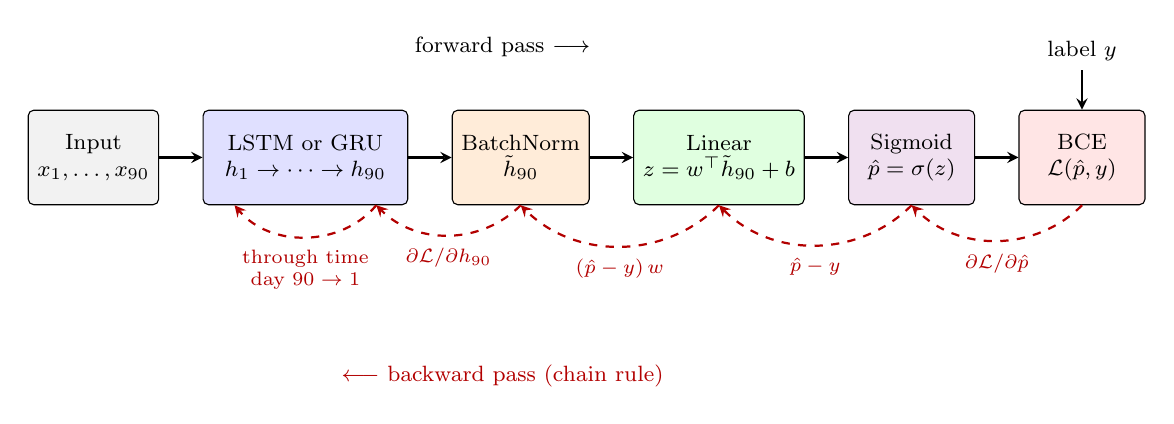
\begin{tikzpicture}[
    op/.style={draw, rounded corners=2pt, minimum height=1.2cm, minimum width=1.6cm, align=center, font=\footnotesize, fill=#1},
    op/.default={gray!10},
    fwd/.style={->, >=stealth, thick},
    bwd/.style={->, >=stealth, thick, red!70!black, dashed},
    grad/.style={font=\scriptsize, red!70!black},
    node distance=0.55cm
]
    % Forward pass
    \node[op] (x) {Input\\$x_1, \dots, x_{90}$};
    \node[op=blue!12, right=of x, minimum width=2.6cm] (rnn) {LSTM or GRU\\$h_1 \to \cdots \to h_{90}$};
    \node[op=orange!15, right=of rnn] (bn) {BatchNorm\\$\tilde h_{90}$};
    \node[op=green!12, right=of bn] (fc) {Linear\\$z = w^\top \tilde h_{90} + b$};
    \node[op=violet!12, right=of fc] (sig) {Sigmoid\\$\hat p = \sigma(z)$};
    \node[op=red!10, right=of sig] (loss) {BCE\\$\mathcal{L}(\hat p, y)$};
    \node[above=0.5cm of loss, font=\footnotesize] (y) {label $y$};

    \draw[fwd] (x) -- (rnn);
    \draw[fwd] (rnn) -- (bn);
    \draw[fwd] (bn) -- (fc);
    \draw[fwd] (fc) -- (sig);
    \draw[fwd] (sig) -- (loss);
    \draw[fwd] (y) -- (loss);
    \node[font=\footnotesize, anchor=south] at ($(x.north)!0.5!(sig.north) + (0,0.55)$) {forward pass $\longrightarrow$};

    % Backward pass: one arc per step, from right to left, labelled with the gradient it carries
    \draw[bwd] (loss.south) to[bend left=45] node[grad, below=1pt] {$\partial \mathcal{L} / \partial \hat p$} (sig.south);
    \draw[bwd] (sig.south) to[bend left=45] node[grad, below=1pt] {$\hat p - y$} (fc.south);
    \draw[bwd] (fc.south) to[bend left=45] node[grad, below=1pt] {$(\hat p - y)\, w$} (bn.south);
    \draw[bwd] (bn.south) to[bend left=45] node[grad, below=1pt] {$\partial \mathcal{L} / \partial h_{90}$} ([xshift=0.9cm]rnn.south);
    \draw[bwd] ([xshift=0.9cm]rnn.south) to[bend left=50] node[grad, below=1pt, align=center] {through time\\day $90 \to 1$} ([xshift=-0.9cm]rnn.south);
    \node[font=\footnotesize, red!70!black, anchor=north] at ($(x.south)!0.5!(sig.south) + (0,-1.9)$) {$\longleftarrow$ backward pass (chain rule)};
\end{tikzpicture}
\caption{Forward and backward passes shared by LSTM and GRU. At the logit the gradient reduces to $\hat p-y$; inside the selected recurrent cell it travels back through the 90 days and its gates.}
\label{fig:w2_backprop}
\end{figure}

The weights are updated with the \textbf{AdamW} optimiser, which computes an adaptive step for each weight from the gradient and applies weight decay separately from that step. It receives two parameters:
\begin{itemize}
    \item \textbf{Learning rate} ($\eta$): how large each update step is.
    \item \textbf{Weight decay} ($\lambda$): shrinks the weights towards zero at every step, which penalises large weights and reduces overfitting.
\end{itemize}

The function \texttt{\_optimizer\_step} (\path{workshops/w2/src/models/recurrent_models/train.py}) performs one update. It calls \texttt{loss.backward()}, clips the gradient norm to 1.0 to limit exploding gradients, and calls \texttt{optimizer.step()}. On GPU the forward pass runs in mixed precision (\texttt{float16}). Neither model uses dropout; overfitting is controlled with weight decay, batch normalisation and early stopping.

\subsection{Hyperparameter Search}

For each recurrent family, Optuna minimises log-loss on the \texttt{tune} partition using the same Tree-structured Parzen Estimator sampler, seed, five-trial budget and search space (Table~\ref{tab:w2_space}). This paired design makes the capacity search comparable rather than favouring one cell with a larger budget.

\begin{table}[H]
\centering
\renewcommand{\arraystretch}{1.3}
\begin{tabular}{|l|l|}
\hline
\textbf{Hyperparameter} & \textbf{Search space} \\ \hline
\texttt{layer\_dim}    & Integer in $[2, 4]$ \\ \hline
\texttt{hidden\_dim}   & $\{32, 64, 128\}$ \\ \hline
Learning rate $\eta$   & $[10^{-4}, 10^{-2}]$, log scale \\ \hline
Weight decay $\lambda$ & $[10^{-6}, 10^{-2}]$, log scale \\ \hline
Batch size             & Fixed at 512 \\ \hline
\end{tabular}
\caption{Shared Optuna search space for LSTM and GRU.}
\label{tab:w2_space}
\end{table}

% ─────────────────────────────────────────────
\section{Training}
% ─────────────────────────────────────────────

\subsection{Data Split}

The February cohort is divided into three disjoint partitions, and the March cohort is kept entirely for the final test (Table~\ref{tab:w2_split}):
\begin{itemize}
    \item \textbf{Fit} (75\%): trains the model.
    \item \textbf{Stop} (12.5\%): validates the model after every epoch for early stopping.
    \item \textbf{Tune} (12.5\%): evaluates each Optuna configuration and selects the decision threshold.
\end{itemize}
Each user is assigned to a partition by a stable hash of their \texttt{msno}, stratified by label, so the split is reproducible and the three partitions keep the same churn rate. Optuna trains each configuration on \texttt{fit}, controls overfitting with \texttt{stop} and evaluates it on \texttt{tune}. The \texttt{test} cohort takes part in no decision.

\begin{table}[H]
\centering
\renewcommand{\arraystretch}{1.3}
\begin{tabular}{|l|l|r|r|r|}
\hline
\textbf{Partition} & \textbf{Cohort} & \textbf{Users} & \textbf{Churners} & \textbf{Churn rate} \\ \hline
\texttt{fit}  & February & 744{,}699 & 47{,}604 & 6.39\% \\ \hline
\texttt{stop} & February & 124{,}117 & 7{,}934  & 6.39\% \\ \hline
\texttt{tune} & February & 124{,}115 & 7{,}933  & 6.39\% \\ \hline
\texttt{test} & March    & 970{,}960 & 87{,}330 & 8.99\% \\ \hline
\end{tabular}
\caption{Partitions used for training, tuning and testing.}
\label{tab:w2_split}
\end{table}

Before training, the numeric channels are clipped at upper quantile limits and standardised with a mean and standard deviation computed only on the days where the channel is defined (active days for listening, payment days for events, days with a known state for states); the binary flags are left unchanged. During the search these parameters are fitted only on \texttt{fit}, so no information from \texttt{stop}, \texttt{tune} or \texttt{test} enters the scaling.

\subsection{Training Procedure}

Each Optuna trial trains one LSTM or GRU on \texttt{fit} with batches of 512 users for at most 40 epochs. After every epoch the loss is computed on \texttt{stop}; if it does not improve for 5 consecutive epochs (\emph{patience}), training stops and the weights of the best epoch are restored. The restored model then predicts \texttt{tune}, and its log-loss is returned to Optuna:
\begin{equation}
\text{log-loss} = -\frac{1}{N} \sum_{i=1}^{N} \Big[ y_i \log \hat{p}_i + (1 - y_i) \log(1 - \hat{p}_i) \Big].
\end{equation}
We use log-loss as the main criterion because it evaluates the quality of the predicted probabilities, not only the final decision.

\subsection{Optuna Results}

All five trials completed for both families. The same first configuration won both searches: two recurrent layers, 32 hidden units, learning rate $2.29\times10^{-3}$ and weight decay $5.37\times10^{-4}$. Table~\ref{tab:w2_best} reports the selected runs. The GRU obtained a slightly lower tuning log-loss (0.14653 versus 0.14674), converged one epoch earlier and required 3{,}840 fewer trainable parameters.

\begin{table}[H]
\centering
\renewcommand{\arraystretch}{1.3}
\begin{tabular}{|l|c|c|c|c|r|c|c|}
\hline
\textbf{Model} & \textbf{Layers} & \textbf{Hidden} & \textbf{$\eta$} & \textbf{$\lambda$} & \textbf{Params} & \textbf{Best ep.} & \textbf{Tune loss} \\ \hline
LSTM & 2 & 32 & $2.29 \times 10^{-3}$ & $5.37 \times 10^{-4}$ & 15{,}457 & 11 & 0.14674 \\ \hline
GRU  & 2 & 32 & $2.29 \times 10^{-3}$ & $5.37 \times 10^{-4}$ & 11{,}617 & 10 & \textbf{0.14653} \\ \hline
\end{tabular}
\caption{Best Optuna configuration for each recurrent family.}
\label{tab:w2_best}
\end{table}

\begin{figure}[H]
\centering
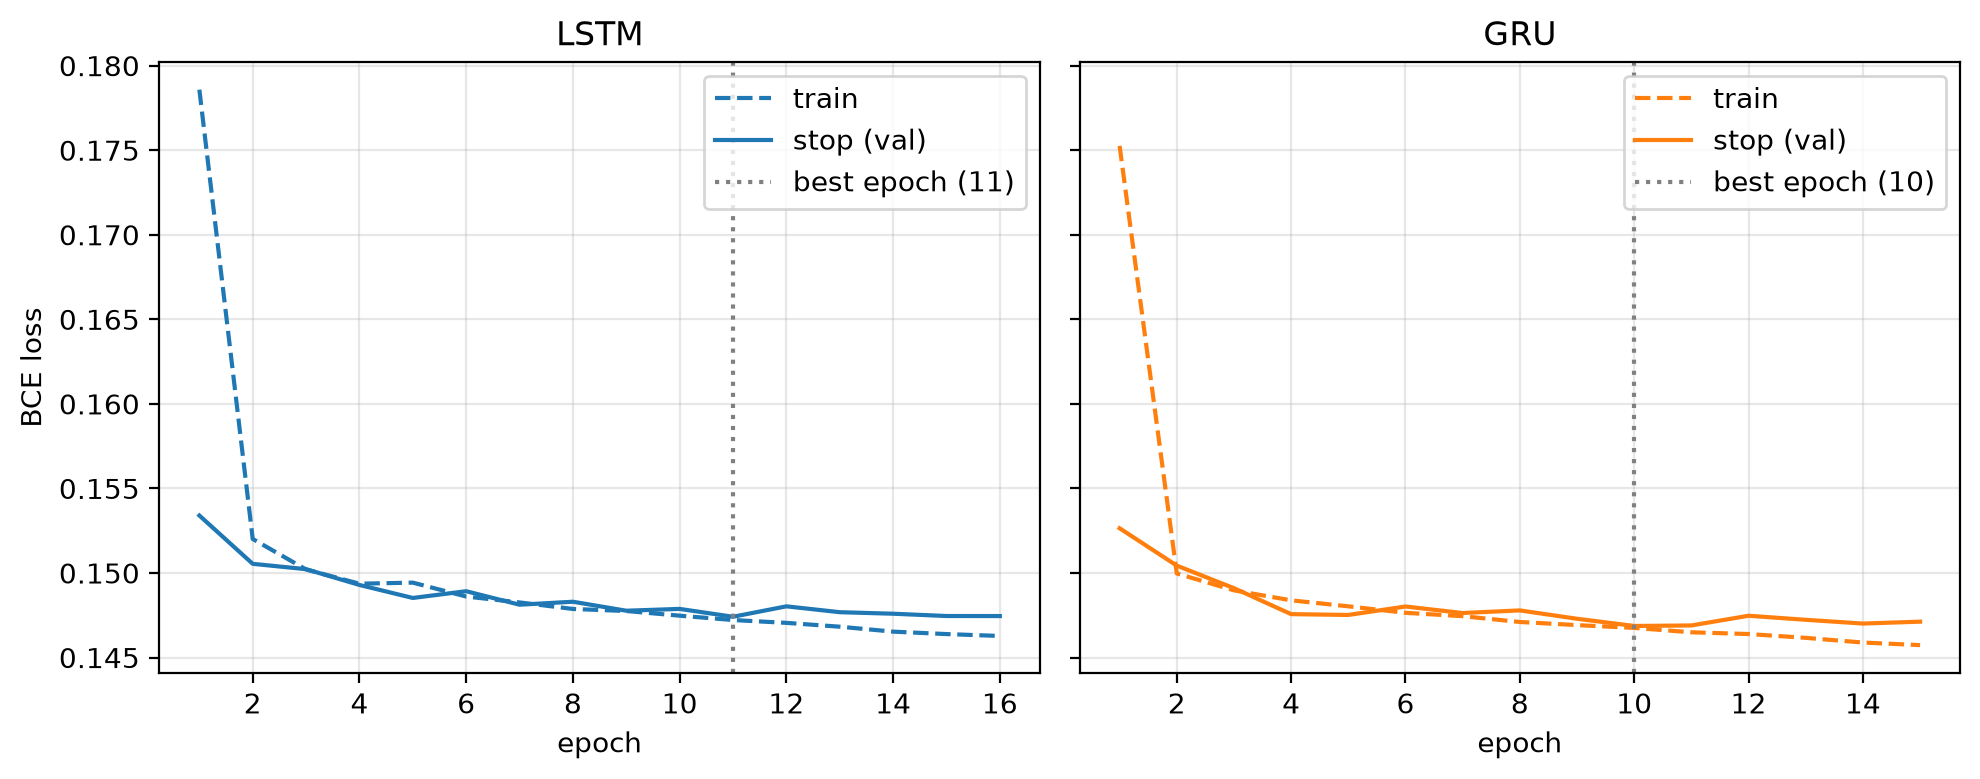
\includegraphics[width=0.8\textwidth]{../../workshops/w2/artifacts/sherlock_w2/comparison/training_history.png}
\caption{Training and early-stopping loss histories of the selected LSTM and GRU trials.}
\label{fig:w2_training_history}
\end{figure}

\paragraph{Decision thresholds.} Each model's threshold is selected independently on \texttt{tune}, in steps of 0.01 from 0.01 to 0.99, to maximise churn-class F1. The selected thresholds are 0.27 for LSTM and 0.24 for GRU. Both are frozen before examining the test cohort.

\paragraph{Final models.} Each selected architecture is retrained on the whole February cohort (992{,}931 users) for its selected number of epochs, with preprocessing refitted on all February data. Each final model then predicts March once.

% ─────────────────────────────────────────────
\section{Test}
% ─────────────────────────────────────────────

\subsection{Metrics}

Both final models are evaluated on the same March cohort (970{,}960 users, 8.99\% churners). Probability metrics (log-loss and Brier score) measure probability quality; ranking metrics (ROC-AUC and average precision) measure ordering; threshold-dependent metrics describe the operating point selected on February. Table~\ref{tab:w2_test} reports the paired results.

\begin{table}[H]
\centering
\renewcommand{\arraystretch}{1.3}
\begin{tabular}{|l|c|c|}
\hline
\textbf{Metric} & \textbf{LSTM (thr. 0.27)} & \textbf{GRU (thr. 0.24)} \\ \hline
Log-loss            & \textbf{0.20384} & 0.20707 \\ \hline
Brier score         & \textbf{0.05412} & 0.05501 \\ \hline
ROC-AUC             & \textbf{0.85030} & 0.84955 \\ \hline
Average precision   & 0.58075 & \textbf{0.58081} \\ \hline
Accuracy            & 0.92714 & \textbf{0.92991} \\ \hline
Balanced accuracy   & \textbf{0.76268} & 0.75433 \\ \hline
Precision (churn)   & 0.60162 & \textbf{0.62837} \\ \hline
Recall (churn)      & \textbf{0.56216} & 0.54023 \\ \hline
Specificity         & 0.96321 & \textbf{0.96842} \\ \hline
F1 (churn)          & \textbf{0.58122} & 0.58097 \\ \hline
F1 (macro)          & 0.77066 & \textbf{0.77137} \\ \hline
MCC                 & 0.54174 & \textbf{0.54482} \\ \hline
Predicted churn rate & 8.40\% & 7.73\% \\ \hline
\end{tabular}
\caption{Test metrics at the model-specific thresholds selected on February. Bold marks the better value for each metric.}
\label{tab:w2_test}
\end{table}

The two models are practically tied in F1 and average precision. LSTM favours recall and probability quality, whereas GRU's lower threshold still produces fewer positive predictions and consequently higher precision, specificity, accuracy and MCC. The default 0.5 threshold is inappropriate for both imbalanced classifiers: it lowers churn F1 to 0.453 for LSTM and 0.402 for GRU.

\subsection{Confusion Matrix}

Figure~\ref{fig:w2_confusion} shows both confusion matrices. LSTM detects 49{,}093 churners (56.2\%) and misses 38{,}237; GRU detects 47{,}178 (54.0\%) and misses 40{,}152. GRU reduces false alarms among loyal users from 32{,}509 to 27{,}902, which explains its precision advantage. The operational choice is therefore explicit: LSTM finds 1{,}915 additional churners at the cost of 4{,}607 additional false positives.

\begin{figure}[H]
\centering
\begin{minipage}{0.49\textwidth}
\centering
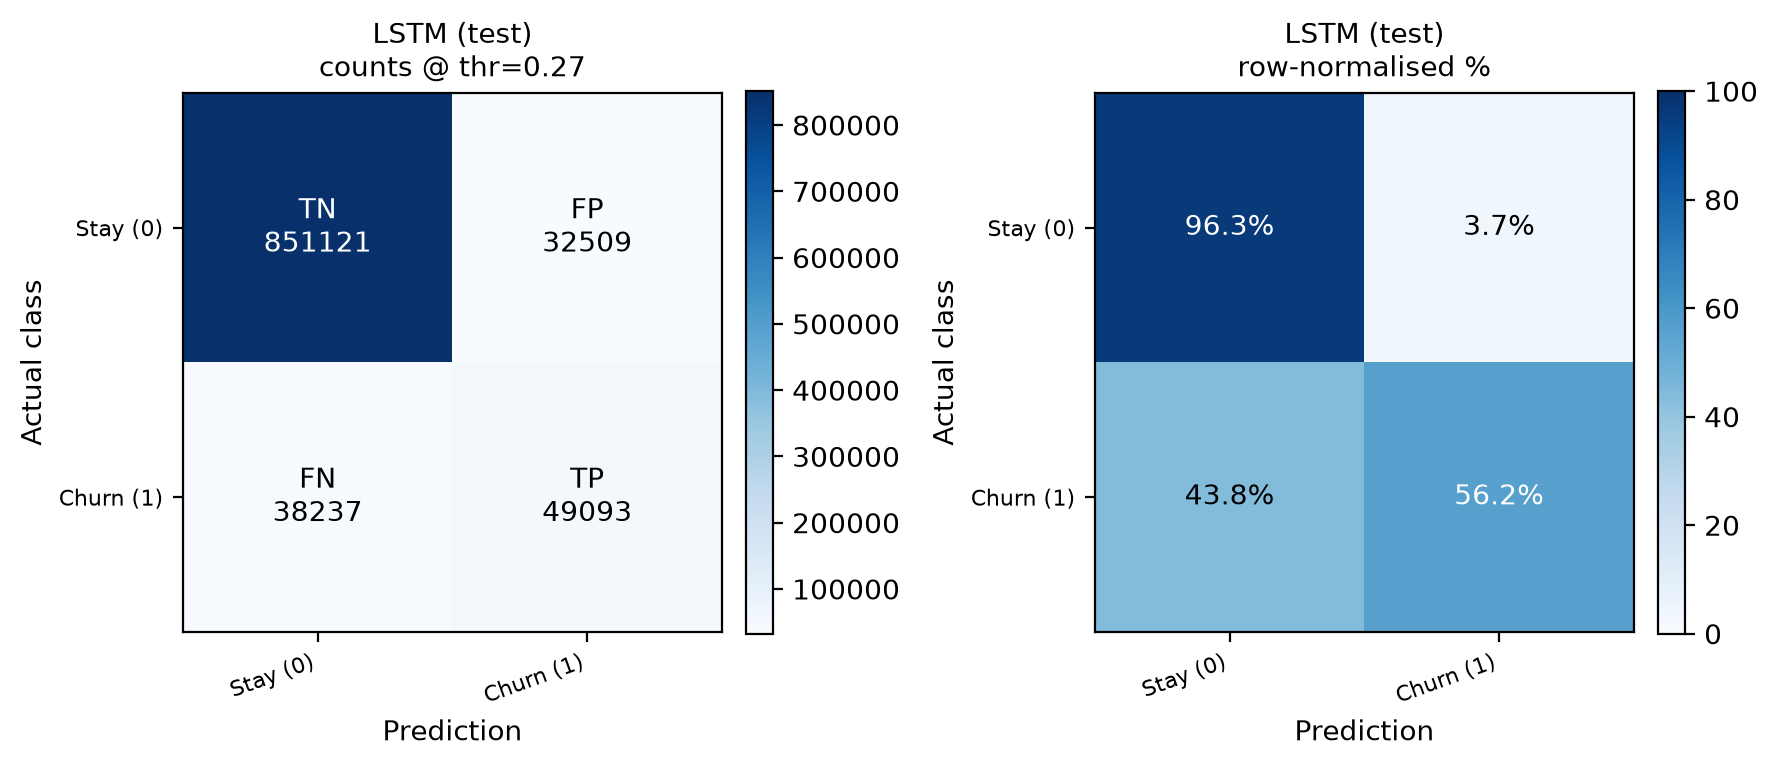
\includegraphics[width=\textwidth]{../../workshops/w2/artifacts/sherlock_w2/lstm/evaluation/figures/confusion/confusion_LSTM_test.png}\\
\small (a) LSTM, threshold 0.27
\end{minipage}
\hfill
\begin{minipage}{0.49\textwidth}
\centering
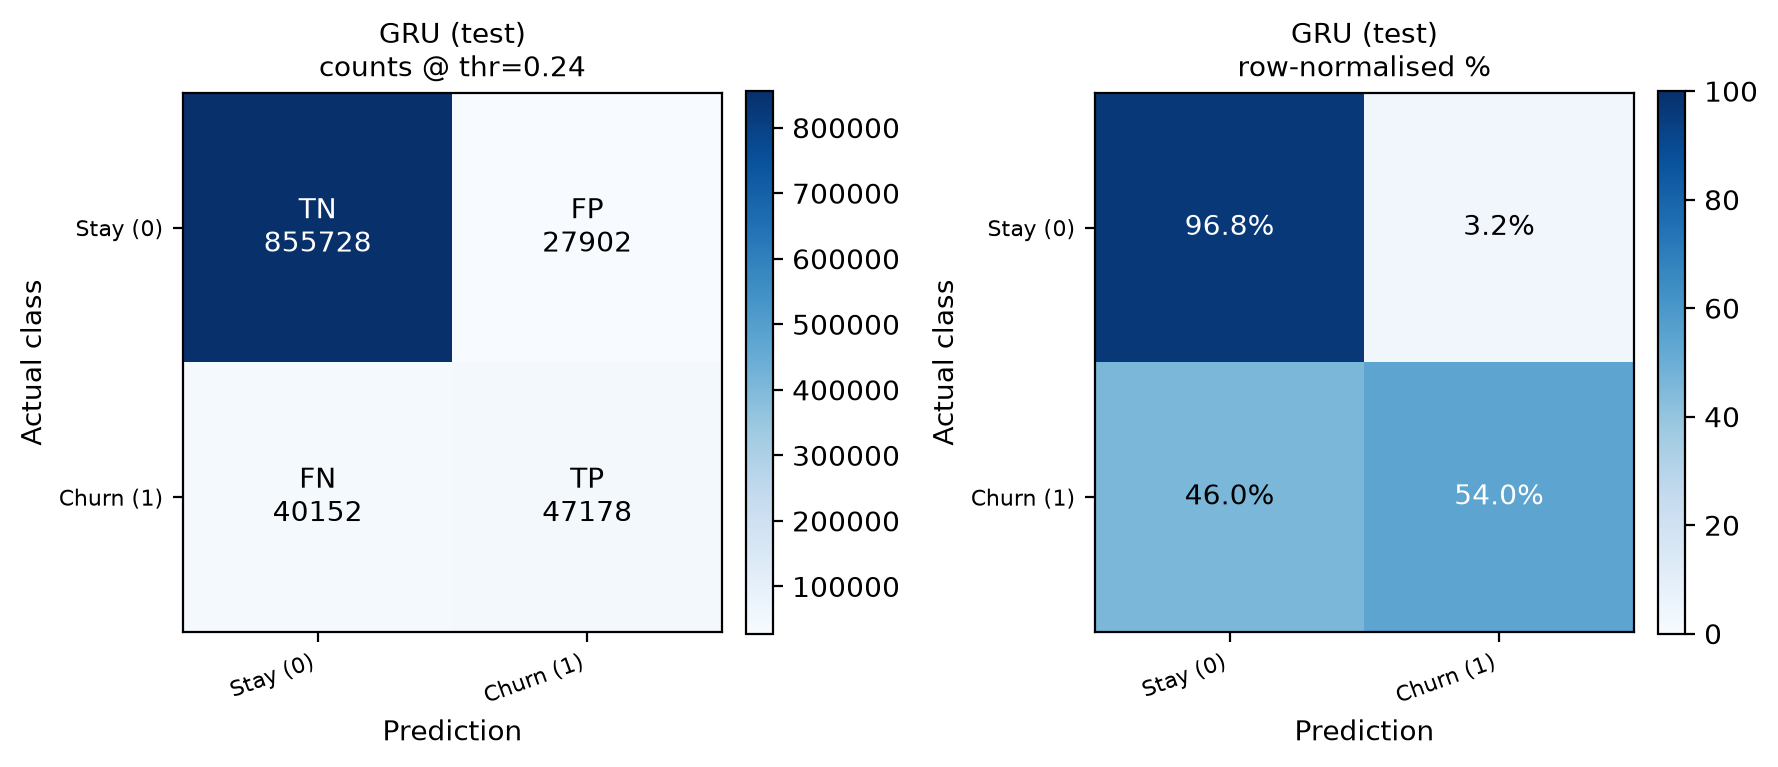
\includegraphics[width=\textwidth]{../../workshops/w2/artifacts/sherlock_w2/gru/evaluation/figures/confusion/confusion_GRU_test.png}\\
\small (b) GRU, threshold 0.24
\end{minipage}
\caption{Confusion matrices on the March test cohort at the model-specific thresholds.}
\label{fig:w2_confusion}
\end{figure}

\subsection{ROC and Precision-Recall Curves}

Figure~\ref{fig:w2_rocpr} overlays the curves. They are almost indistinguishable: the LSTM has a 0.00075 advantage in ROC-AUC, while the GRU has a 0.00006 advantage in average precision. Both are far above the 8.99\% precision baseline of a random ranking.

\begin{figure}[H]
\centering
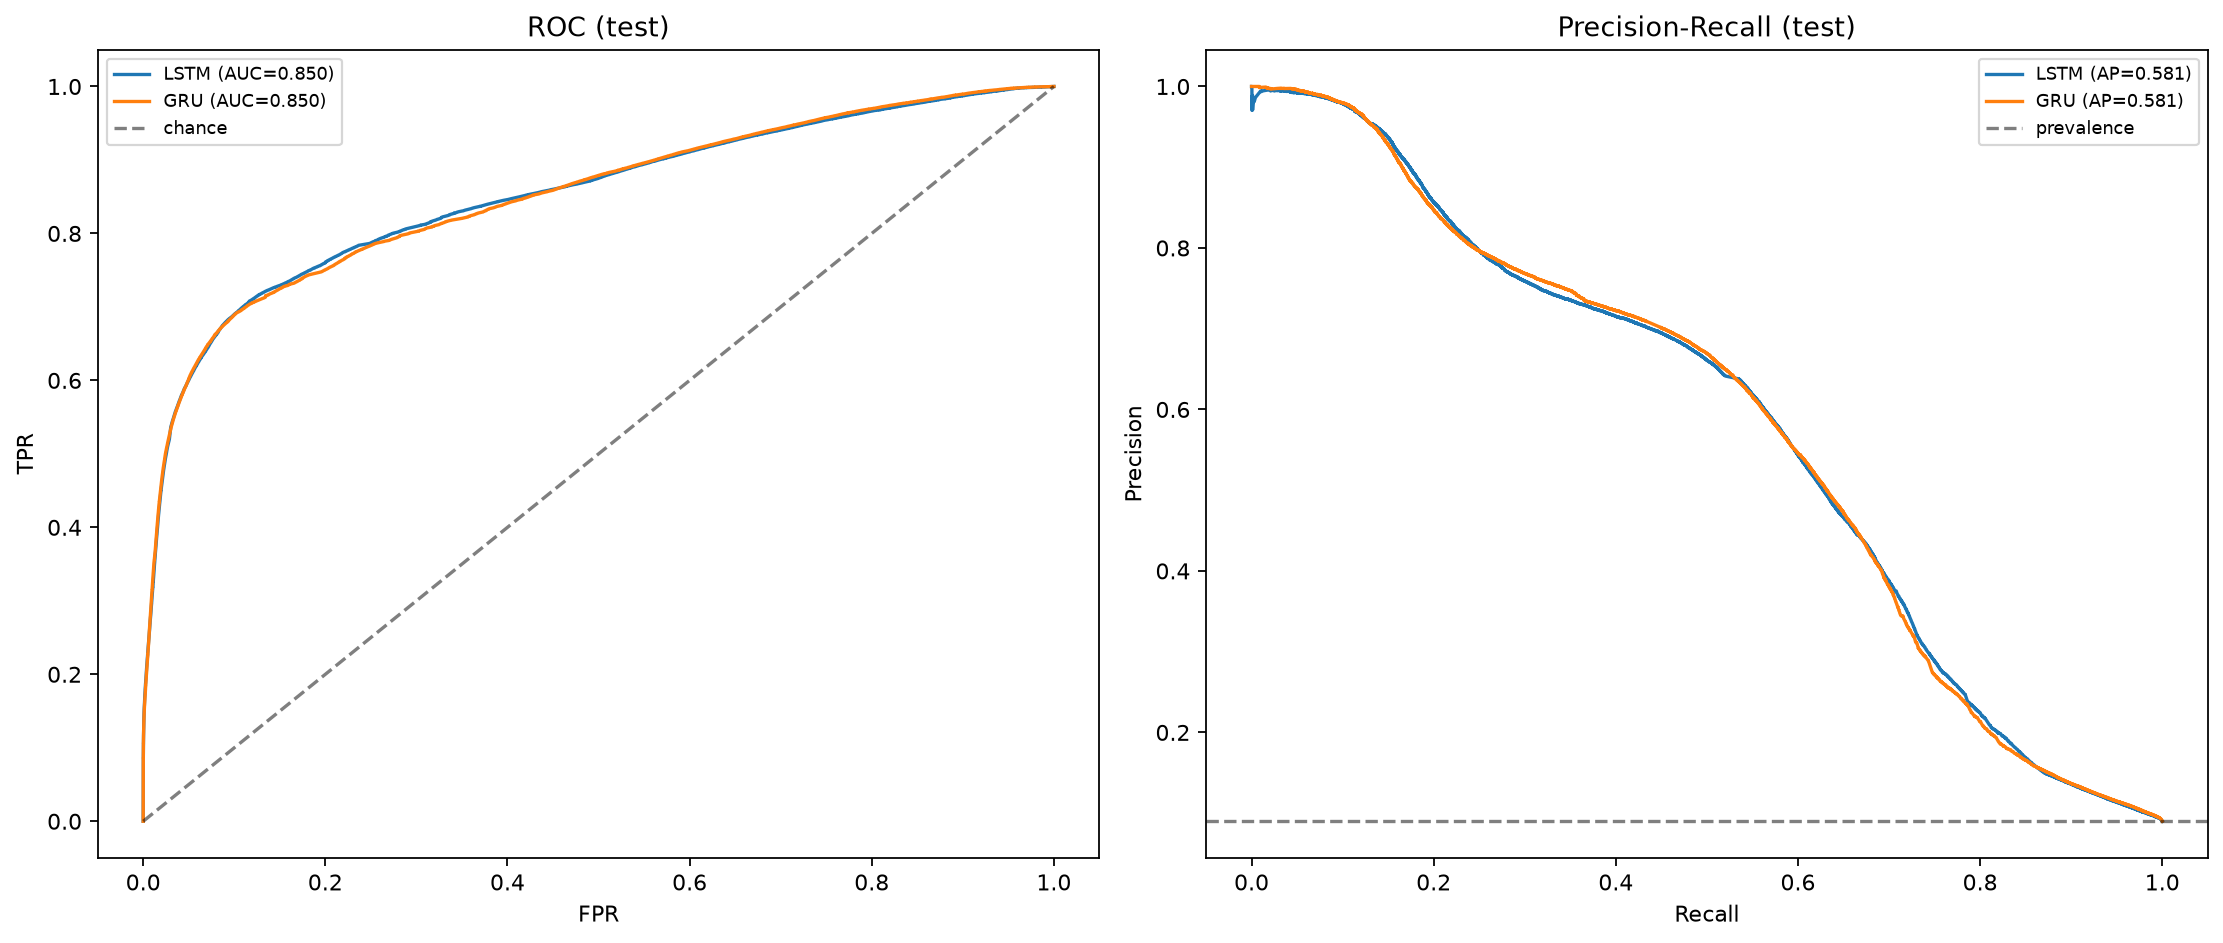
\includegraphics[width=\textwidth]{../../workshops/w2/artifacts/sherlock_w2/comparison/roc_pr_comparison.png}
\caption{ROC and precision-recall curves for LSTM and GRU on the March test cohort.}
\label{fig:w2_rocpr}
\end{figure}

\subsection{Calibration}

Figure~\ref{fig:w2_calibration} shows each reliability diagram and score distribution. Both models underestimate churn in March, consistent with the prevalence increase from 6.4\% in February to 9.0\% in March. LSTM nevertheless has the lower log-loss and Brier score, so its probabilities are better calibrated overall. Neither model was recalibrated after the temporal shift.

\begin{figure}[H]
\centering
\begin{minipage}{0.49\textwidth}
\centering
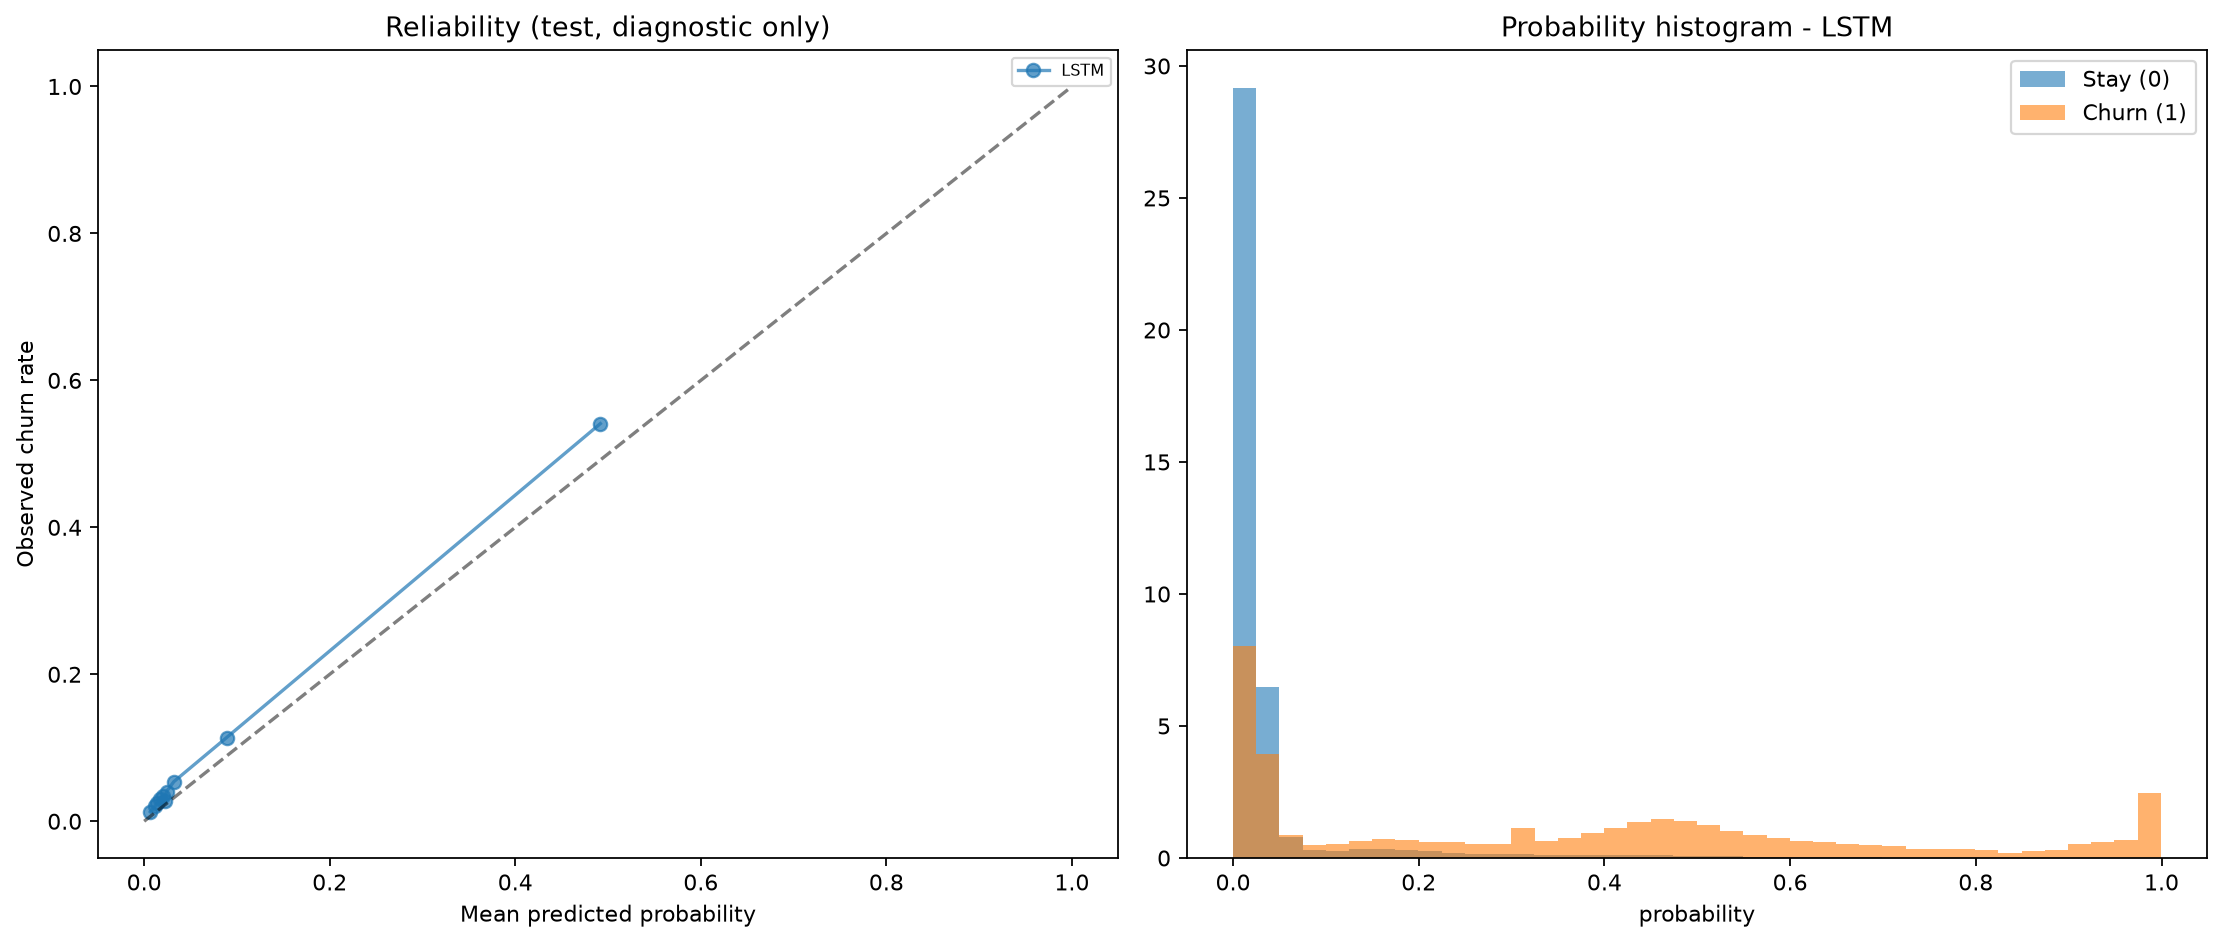
\includegraphics[width=\textwidth]{../../workshops/w2/artifacts/sherlock_w2/lstm/evaluation/figures/curves/calibration_hist.png}\\
\small (a) LSTM
\end{minipage}
\hfill
\begin{minipage}{0.49\textwidth}
\centering
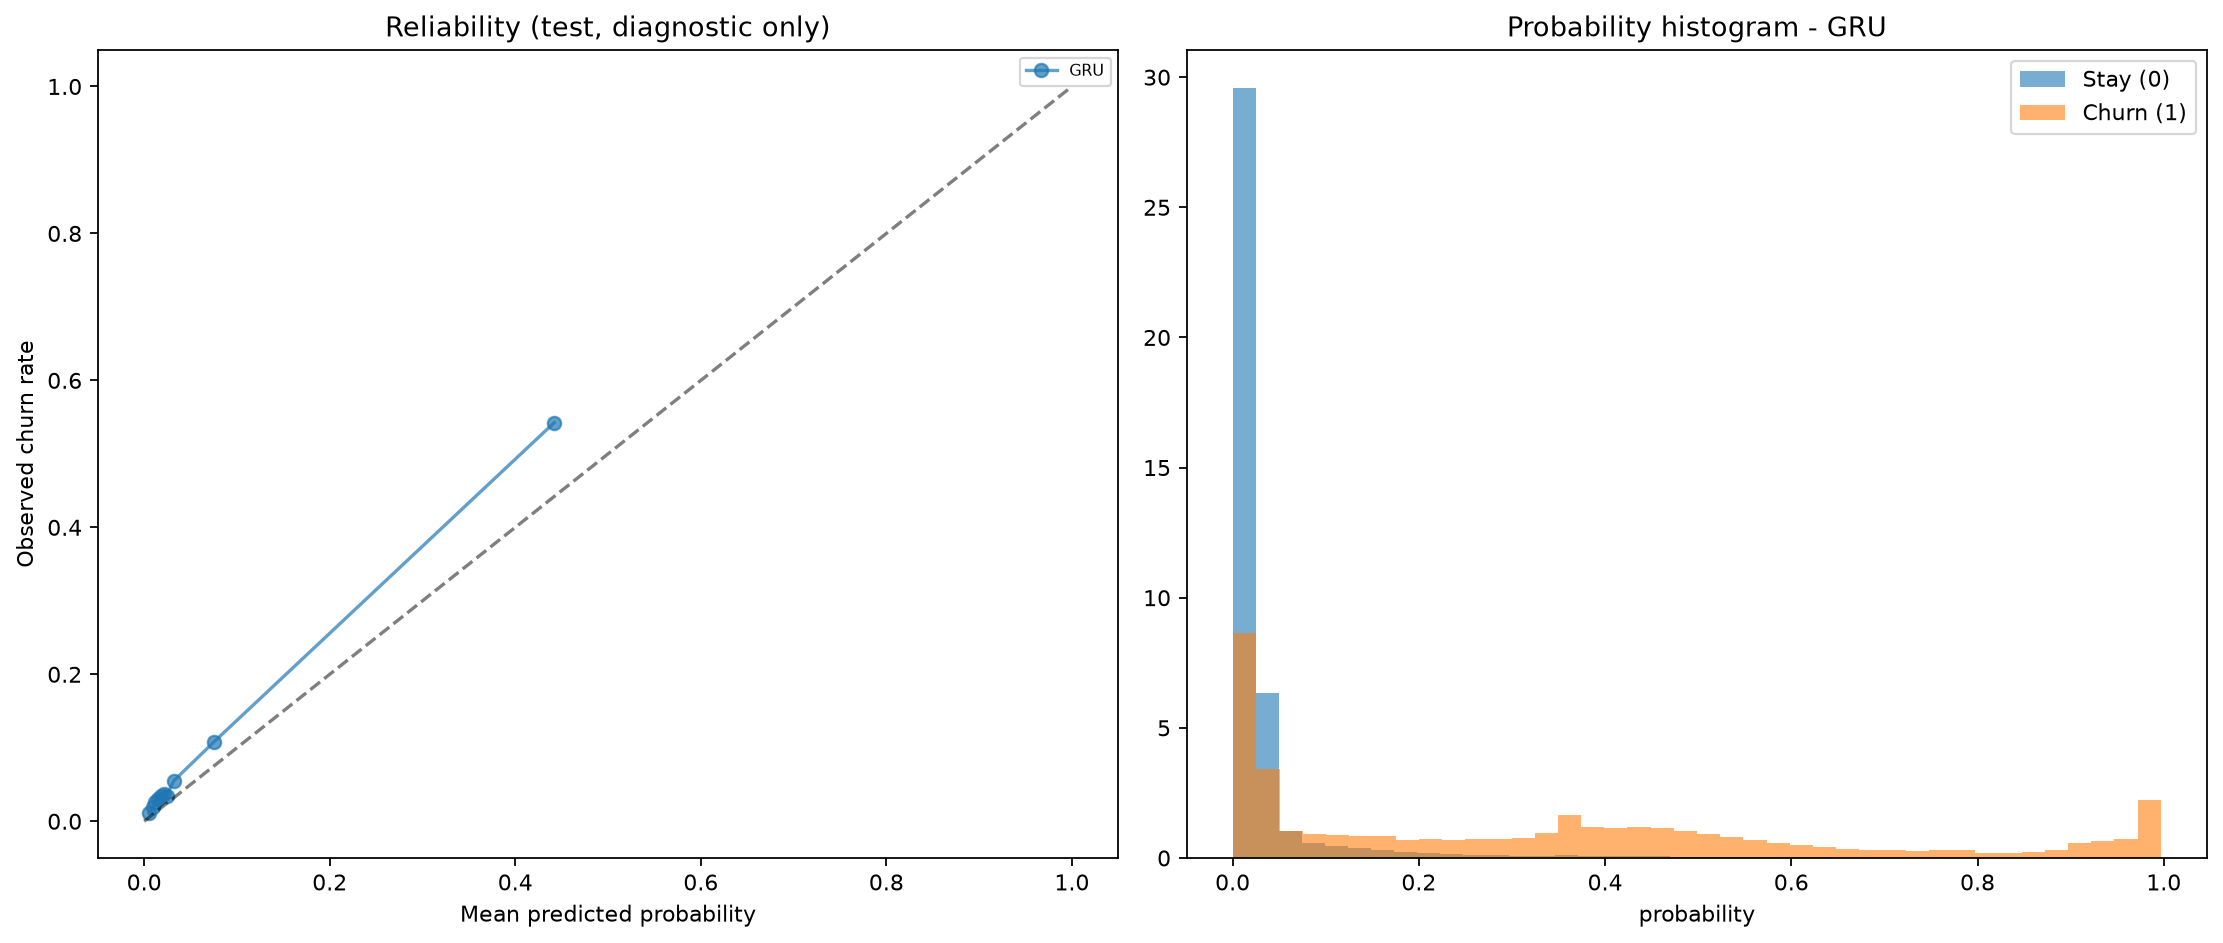
\includegraphics[width=\textwidth]{../../workshops/w2/artifacts/sherlock_w2/gru/evaluation/figures/curves/calibration_hist.png}\\
\small (b) GRU
\end{minipage}
\caption{Reliability diagrams and predicted-probability distributions on the March test cohort.}
\label{fig:w2_calibration}
\end{figure}

\subsection{Statistical and Operational Comparison}

Because a dataset of almost one million users can make very small differences statistically detectable, we report paired 95\% bootstrap confidence intervals and interpret effect size as well as significance (Table~\ref{tab:w2_significance}). DeLong's paired test also detects the LSTM's ROC-AUC advantage ($\Delta=0.00075$, $z=2.47$, $p=0.0134$). However, the magnitude is operationally negligible. The bootstrap intervals show no reliable difference in average precision or F1. The clear difference is log-loss: LSTM improves it by 0.00323, although the practical gain remains modest.

\begin{table}[H]
\centering
\small
\renewcommand{\arraystretch}{1.25}
\begin{tabular}{|l|c|c|c|c|}
\hline
\textbf{Metric} & \textbf{LSTM (95\% CI)} & \textbf{GRU (95\% CI)} & \textbf{$\Delta$ LSTM--GRU (95\% CI)} & \textbf{Sig.} \\ \hline
ROC-AUC & 0.8503 [0.8487, 0.8519] & 0.8495 [0.8480, 0.8511] & 0.00075 [0.0001, 0.0014] & Yes \\ \hline
Average precision & 0.5808 [0.5774, 0.5840] & 0.5808 [0.5774, 0.5842] & $-0.00006$ [$-0.0009$, 0.0006] & No \\ \hline
F1 (churn) & 0.5812 [0.5783, 0.5839] & 0.5810 [0.5780, 0.5837] & 0.00024 [$-0.0009$, 0.0014] & No \\ \hline
Log-loss & 0.2038 [0.2026, 0.2051] & 0.2071 [0.2058, 0.2084] & $-0.00323$ [$-0.0034$, $-0.0030$] & Yes \\ \hline
\end{tabular}
\caption{Paired bootstrap comparison on March. For log-loss, a negative difference favours LSTM.}
\label{tab:w2_significance}
\end{table}

The models also produce nearly identical ranked contact lists (Figure~\ref{fig:w2_gain}). If the retention team contacts the top 5\% of users, LSTM captures 39.82\% of all churners (lift 7.96) and GRU captures 40.14\% (lift 8.03). At 10\%, they capture 60.17\% and 60.32\%, respectively. LSTM becomes slightly better at 20\% and 30\% contact budgets. Thus GRU is marginally preferable for a very narrow campaign, but the difference is less than 0.4 percentage points.

\begin{figure}[H]
\centering
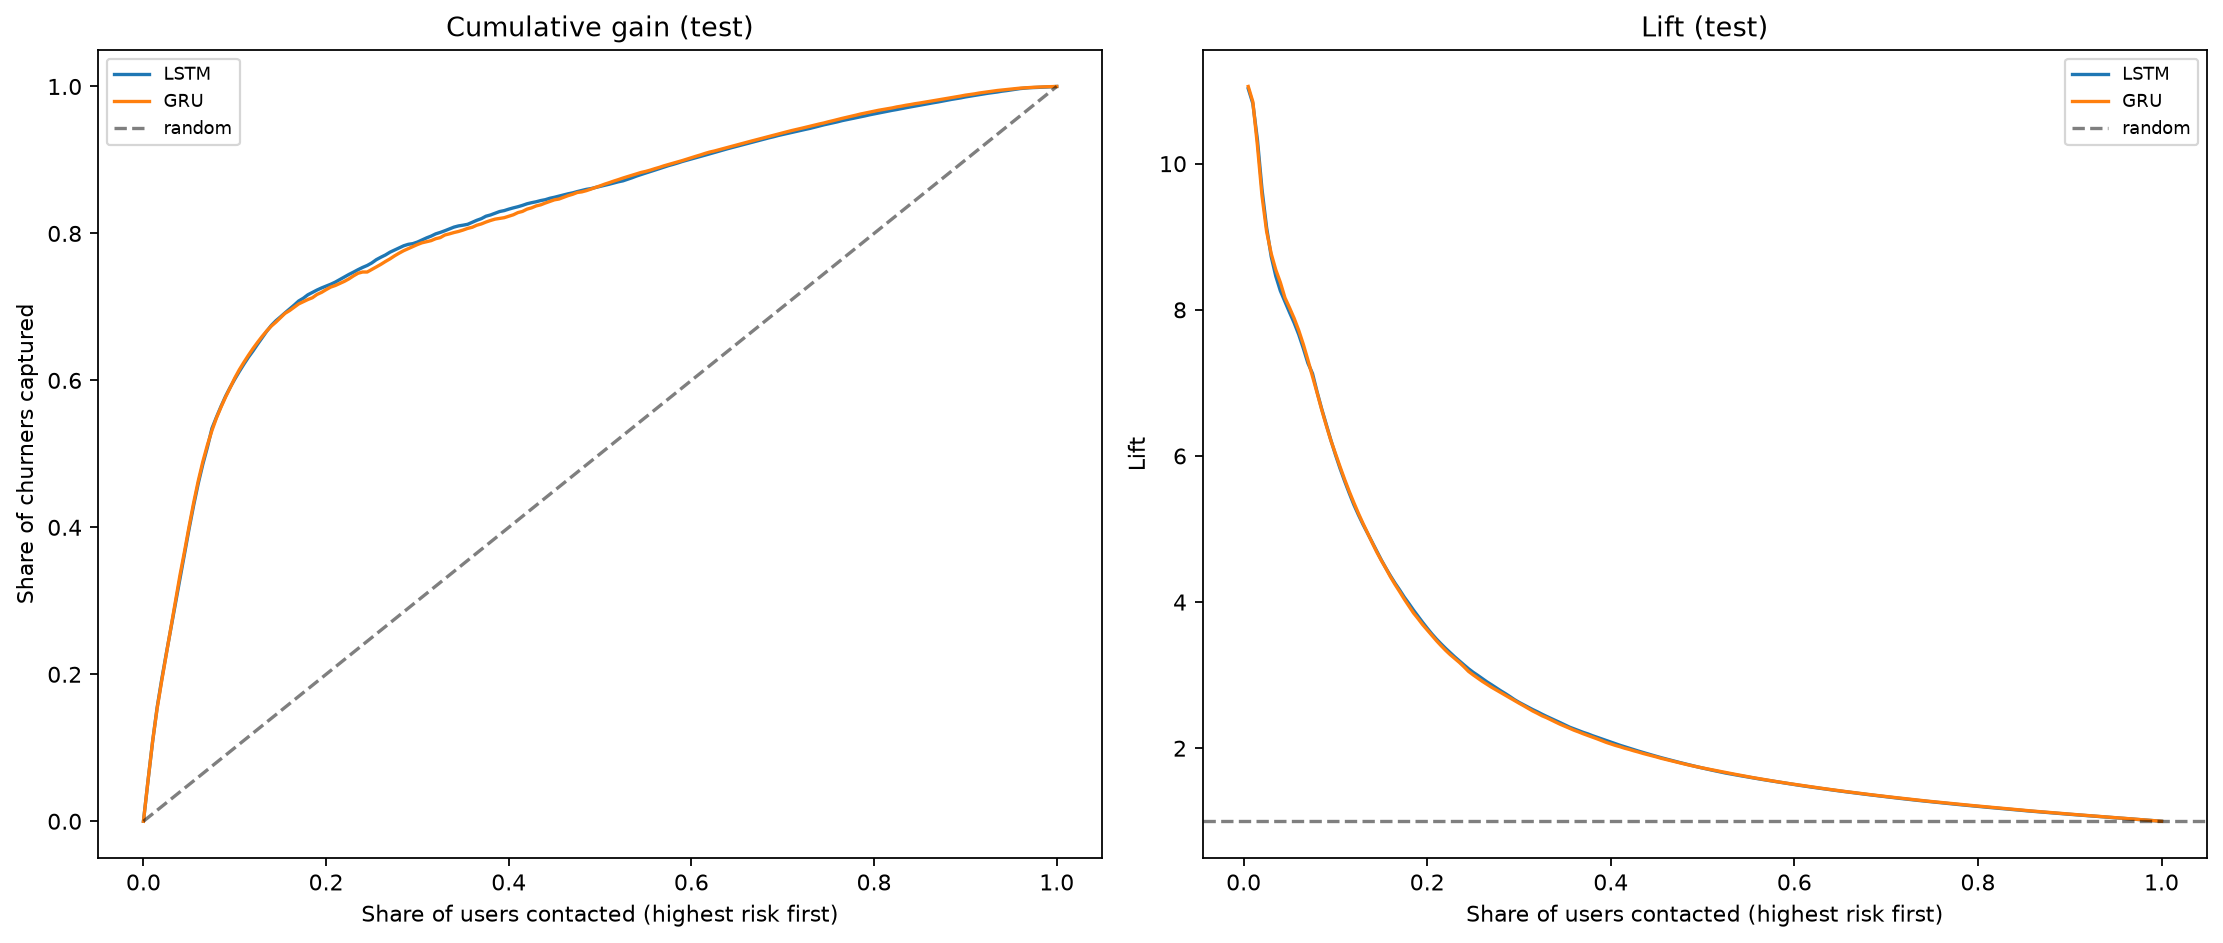
\includegraphics[width=0.9\textwidth]{../../workshops/w2/artifacts/sherlock_w2/comparison/gain_lift_comparison.png}
\caption{Cumulative gain and lift for ranked retention campaigns.}
\label{fig:w2_gain}
\end{figure}

\paragraph{Efficiency.} At the selected architecture, GRU uses 11{,}617 parameters versus 15{,}457 for LSTM, a 24.8\% reduction, and takes 16.62 versus 18.11 seconds per epoch, an 8.2\% reduction in the recorded run. Given their virtually equal ranking and classification performance, GRU offers the better efficiency--performance trade-off; LSTM is preferable when probability quality or maximum recall is the priority.

\subsection{Comparison with Workshop 1}

Table~\ref{tab:w2_vs_w1} adds both recurrent models to the three tabular models from Workshop~1. All are evaluated on March after choosing thresholds on February. The tabular models use 59 engineered features, demographics and complete transaction history; LSTM and GRU use only the 90-day sequence.

\begin{table}[H]
\centering
\small
\setlength{\tabcolsep}{3pt}
\renewcommand{\arraystretch}{1.3}
\begin{tabular}{|l|c|c|c|c|c|c|c|c|c|}
\hline
\textbf{Model} & \textbf{Thr.} & \textbf{Log-loss} & \textbf{Brier} & \textbf{AUC} & \textbf{AP} & \textbf{Prec.} & \textbf{Recall} & \textbf{F1} & \textbf{MCC} \\ \hline
Logistic reg. (W1) & 0.28 & 0.2126 & 0.0564 & 0.8445 & 0.5553 & 0.5811 & 0.5343 & 0.5567 & 0.5155 \\ \hline
Random forest (W1)       & 0.26 & \textbf{0.2032} & 0.0548 & \textbf{0.8632} & \textbf{0.5933} & \textbf{0.6379} & 0.5385 & \textbf{0.5840} & \textbf{0.5490} \\ \hline
XGBoost (W1)             & 0.88 & 0.4886 & 0.1498 & 0.8520 & 0.5882 & 0.6094 & \textbf{0.5424} & 0.5740 & 0.5356 \\ \hline
LSTM (W2)                & 0.27 & 0.2038 & \textbf{0.0541} & 0.8503 & 0.5808 & 0.6016 & \textbf{0.5622} & 0.5812 & 0.5417 \\ \hline
GRU (W2)                 & 0.24 & 0.2071 & 0.0550 & 0.8495 & 0.5808 & 0.6284 & 0.5402 & 0.5810 & 0.5448 \\ \hline
\end{tabular}
\caption{Test metrics on March for Workshop~1 tabular models and Workshop~2 recurrent models. Best value per column is bold.}
\label{tab:w2_vs_w1}
\end{table}

Random forest retains the best ROC-AUC, average precision, F1 and MCC, but LSTM now has the best Brier score and recall and is only 0.0006 worse in log-loss. Both recurrent models outperform logistic regression in ranking and F1, and greatly outperform the poorly calibrated Workshop~1 XGBoost in log-loss. The comparison also shows that cell choice is much less important than representation: LSTM and GRU differ from each other far less than either differs from the tabular models.

% ─────────────────────────────────────────────
\section{Conclusions}
% ─────────────────────────────────────────────

\paragraph{LSTM versus GRU.} Both gated recurrent cells extract almost the same predictive signal from the daily sequence: F1 differs by only 0.00024 and average precision by 0.00006. LSTM yields better probabilities and detects more churners, while GRU produces fewer false alarms, uses 24.8\% fewer parameters and trains 8.2\% faster per epoch. Therefore there is no universally superior cell: LSTM is the choice for probability quality and recall, whereas GRU is the parsimonious choice when compute, model size or contact precision matters.

\paragraph{Relation with Workshop 1.} Workshop~1 summarises each subscriber into 59 hand-crafted features, while both recurrent models learn from a $90\times20$ daily sequence. Under the same temporal protocol, LSTM and GRU approach the random forest (F1 0.581 versus 0.584) without demographics or full-history aggregates. This supports the value of temporal order, but the remaining ranking gap suggests that tenure, demographics and older payment history still add information beyond the 90-day window.

\paragraph{How the sequence captures behaviour.} The daily tensor preserves patterns compressed by monthly aggregates: a user who stops listening during the last two weeks, cancellation followed by inactivity, or expiry without renewal. Both cells can preserve or discard earlier information through gates; LSTM uses separate memory and hidden states, whereas GRU performs the same role with a single state. We did not attribute predictions to individual days or channels, so claims about which pattern each network actually uses require a future interpretability analysis.

\paragraph{Why no further experiments are possible.} The main limitation is the dataset itself. The competition publishes official churn labels for only two months: February 2017 (\texttt{train.csv}) and March 2017 (\texttt{train\_v2.csv}). A user is labelled as churn when their membership expires in the target month and they do not subscribe again within the following 30 days, so labelling a month requires the transactions of the next 30 days. Since the published transactions and logs end on 2017-03-31, no later month (April 2017 onwards) can be labelled. Earlier months, such as January 2017 or December 2016, could in principle be labelled by applying the official labelling rule to the transactions, and the listening history before the window is available since 2015. However, our reconstruction of that rule, a port of the official \texttt{WSDMChurnLabeller.scala}, agrees with the official labels for only 98.8\% of the February users and 97.0\% of the March users, and about 137{,}000 official users per month cannot be reconstructed from the published transactions. Labels for other months would therefore be noisier than the official ones and would not define the same cohorts, so a model trained or tested on them would not be comparable with the results reported here. For this reason the evaluation is limited to one training month and one test month, and we cannot measure how stable the model is across several months.

\begin{thebibliography}{9}

\bibitem{chung2014}
Chung, J., Gulcehre, C., Cho, K., \& Bengio, Y. (2014).
\textit{Empirical evaluation of gated recurrent neural networks on sequence modeling}.
arXiv:1412.3555. \url{https://doi.org/10.48550/arXiv.1412.3555}

\bibitem{kkbox2017}
KKBOX. (2017).
\textit{WSDM--KKBox's Churn Prediction Challenge} [Data set and competition].
Kaggle. \url{https://www.kaggle.com/competitions/kkbox-churn-prediction-challenge}

\end{thebibliography}

\end{document}
